% !TEX TS-program = pdflatex
% !TEX encoding = UTF-8 Unicode

% This file is a template using the "beamer" package to create slides for a talk or presentation
% - Giving a talk on some subject.
% - The talk is between 15min and 45min long.
% - Style is ornate.

% MODIFIED by Jonathan Kew, 2008-07-06
% The header comments and encoding in this file were modified for inclusion with TeXworks.
% The content is otherwise unchanged from the original distributed with the beamer package.

\documentclass{beamer}


% Copyright 2004 by Till Tantau <tantau@users.sourceforge.net>.
%
% In principle, this file can be redistributed and/or modified under
% the terms of the GNU Public License, version 2.
%
% However, this file is supposed to be a template to be modified
% for your own needs. For this reason, if you use this file as a
% template and not specifically distribute it as part of a another
% package/program, I grant the extra permission to freely copy and
% modify this file as you see fit and even to delete this copyright
% notice. 


\mode<presentation>
{
  \usetheme{Warsaw}
  % or ...
  \usecolortheme{beaver}

  \setbeamercovered{transparent}
  % or whatever (possibly just delete it)
}

\usepackage[english]{babel}
% or whatever

\usepackage[utf8]{inputenc}
% or whatever

\usepackage {wasysym}

\usepackage{times}
\usepackage[T1]{fontenc}
% Or whatever. Note that the encoding and the font should match. If T1
% does not look nice, try deleting the line with the fontenc.
\usepackage{colortbl}

\usepackage{subfig}

\title{Assignment 3}

\subtitle
{Automated Reasoning in AI 2011} % (optional)

\author{Armon Toubman, Torec Luik}

\begin{document}

\begin{frame}
  \titlepage
\end{frame}

%\begin{frame}{Outline}
%  \tableofcontents
%\end{frame}


% Since this a solution template for a generic talk, very little can
% be said about how it should be structured. However, the talk length
% of between 15min and 45min and the theme suggest that you stick to
% the following rules:  

% - Exactly two or three sections (other than the summary).
% - At *most* three subsections per section.
% - Talk about 30s to 2min per frame. So there should be between about
%   15 and 30 frames, all told.

%\section{Introduction}

\begin{frame}{Description Logic}

\begin{figure}[htbp]
\begin{center}
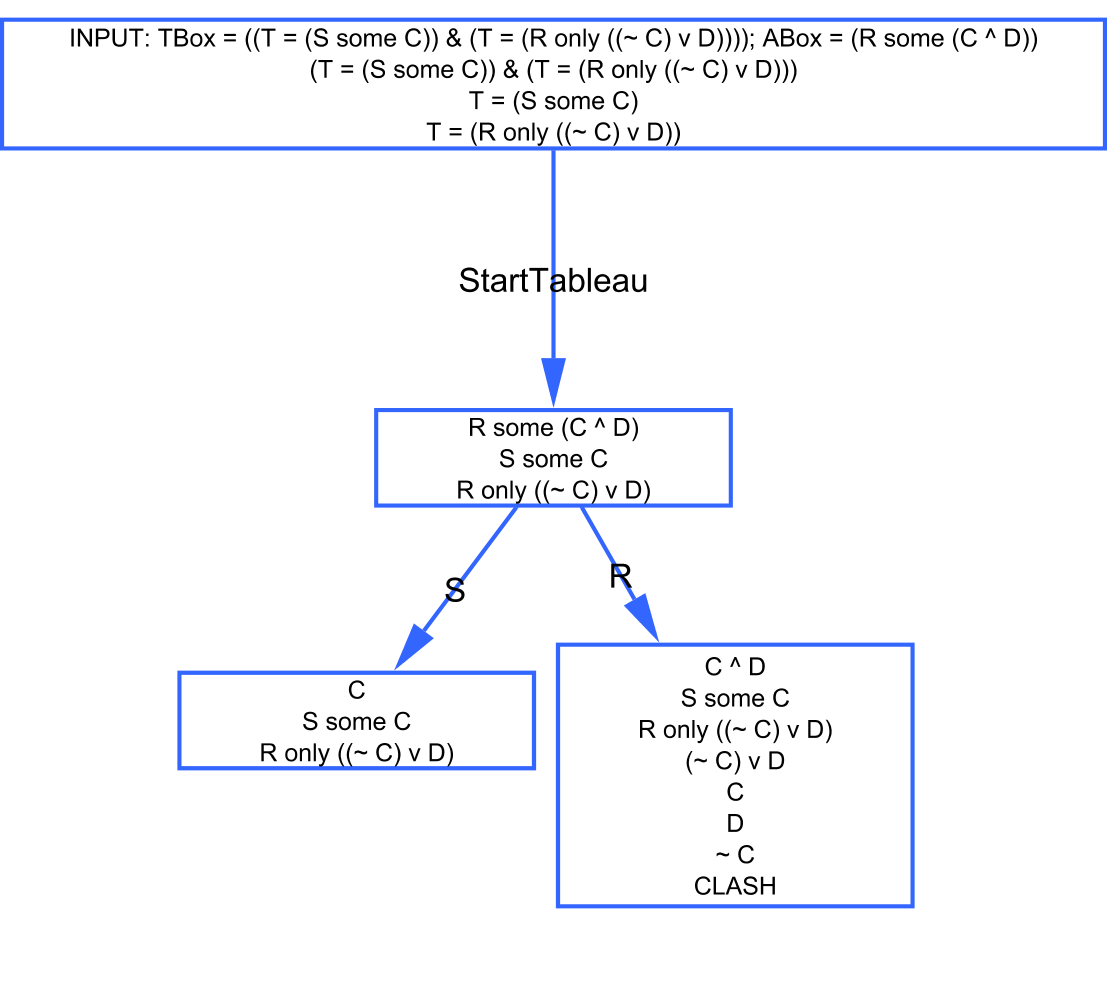
\includegraphics[scale=0.2]{figure1.png}
\end{center}
\end{figure}

\end{frame}

%\section{Tableau algorithm}

%\subsection{Operators}

\begin{frame}{Operators}

\begin{table}[h]
\begin{center}

\scalebox{0.75}{
\begin{tabular}{l c c c c c c}
$\mathcal{ALC}$ syntax & $\neg C$ & $C \sqcap D$ & $C \sqcup D$ & $\exists r.C$ & $\forall r.C$ & $\top \equiv D$\\
LoTREC connective & \texttt{not} $C$ & \texttt{and} $C D$ & \texttt{or} $C D$ & \texttt{some} $r$ $C$ & \texttt{only} $r$ $C$ & \texttt{tbox} $D$\\
LoTREC display & $\sim$ $C$ & $C$ $^\wedge$ $D$ & $C$ v $D$ & $r$ some $C$ & $r$ only $C$ & $\top$ = $D$\\
\end{tabular}
}

\end{center}
\end{table}

\begin{table}[h]
\begin{center}

\scalebox{0.9}{
\begin{tabular}{l c c}
LoTREC connective & \texttt{add} $\phi$ $\psi$ & \texttt{input} $\mathcal{T}$ $C$\\
LoTREC display & $\phi$ \& $\psi$ & INPUT: TBox = $\mathcal{T}$; ABox = $C$\\
\end{tabular}
}

\end{center}
\end{table}

\end{frame}

\begin{frame}{Example formula}

\begin{table}[h]
\begin{center}

\scalebox{1}{
\begin{tabular}{c}
(\{$\top \equiv \exists s.C$, $\top \equiv \forall r.(\neg C \sqcup D)$\}, $\exists r.(C \sqcap D)$)\\
\texttt{input add tbox some S C tbox only R or not C D}\\
\texttt{some R and C D}\\
\end{tabular}
}

\end{center}
\end{table}

\end{frame}

%\subsection{Rules}

% met strategy uitleggen

%\subsection{Strategy}

\begin{frame}{Strategy}

\begin{block}{Efficient Strategy}
repeat [ Initiate AddFromList TBoxRule ] end\\
repeat\\
....firstRule\\
........Clash\\
........FalsumRule\\
........TruthRule\\
........OnlyRule\\
........AndRule\\
........OrRule\\
........allRules [ Block SomeRule TBoxRule ] end \\
....end\\
end
\end{block}

\end{frame}

\begin{frame}{Ordering}
\begin{block}{Efficient Strategy}
\uncover<1>{repeat [ Initiate AddFromList TBoxRule ] end\\}
\uncover<1->{repeat\\}
\uncover<2->{....firstRule\\}
\uncover<2>{........Clash\\}
\uncover<3>{........FalsumRule\\}
\uncover<3>{........TruthRule\\}
\uncover<5>{........OnlyRule\\}
\uncover<5>{........AndRule\\}
\uncover<5>{........OrRule\\}
\uncover<4>{........allRules [ Block SomeRule TBoxRule ] end \\}
\uncover<2->{....end\\}
\uncover<1->{end}
\end{block}

\end{frame}

\begin{frame}{Ordering - Example}

\begin{table}[h]
\begin{center}

\scalebox{1}{
\begin{tabular}{c}
($A$, $\neg A$, $B\sqcap (C \sqcup D)$, $\exists X. A \sqcup B$)\\
\texttt{add add add A not A and B or C D some X or A B}\\
\end{tabular}
}

\end{center}
\end{table}

\end{frame}

%\section{Reasoning problems}

% skip?

%\section{Strategies}

\begin{frame}{Wrong Blocking - Problem}

The blocking rule must be used only when no other rules, except for possibly the existential rule, 

are applicable on the branch.

Completeness is lost when this is violated.

\end{frame}

\begin{frame}{Wrong Blocking - Strategy}

\begin{block}{Wrong Blocking}
repeat [ Initiate AddFromList TBoxRule ] end\\
repeat\\
....firstRule\\
\alert<1>{........Block SomeRule TBoxRule\\}
........TruthRule\\
........FalsumRule\\
........OnlyRule\\
........AndRule\\
........OrRule\\
........Clash\\
....end\\
end
\end{block}

\end{frame}

\begin{frame}{Wrong Blocking - Example}

\begin{itemize}[<+->]
\item Blocking rule is applied before others. 
\item Use of Some rule is inhibited prematurely.
\item Algorithm is falsly satisfied.
\item Node has to be equal to an ancestor.
\item Difference with ancestor might be applicability of the Only rule
\begin{itemize}
    \item Only rule provides, e.g. "some A B".
    \item Some rule should have provided "B" to "A".
    \item If "A" would then already contain "$\neg B$", CLASH!
\end{itemize}
\end{itemize}

\end{frame}

%\section{Extensions}

\begin{frame}{Extensions}

\begin{itemize}
\item Transitive roles
\item Role hierarchies
\end{itemize}

\end{frame}

\begin{frame}{Transitive roles}

\begin{table}[h]
\begin{center}
\begin{tabular}{l c}
LoTREC connective & \texttt{trans} $C$ \\
LoTREC display & $+C$ \\
\end{tabular}
\end{center}
\end{table}

\begin{table}[h]
\begin{center}
\scalebox{0.8}{
\begin{tabular}{l l}
\texttt{TransitiveRoleSome} & \\
\hline
Conditions: & \texttt{hasElement node trans \_t} \\
 & \texttt{hasElement node some \_t some \_t some \_b} \\
Actions: & \texttt{add node some \_t \_b} \\
\hline
\end{tabular}
}
\end{center}
\end{table}

\end{frame}

\begin{frame}{Transitive roles example}

\begin{table}[h]
\begin{center}
\begin{tabular}{l l}
TBox & $\exists{}hasPart.(\exists{}hasPart.(\exists{}hasPart.Component))$ \\
ABox & $\exists{}hasPart.Component$ \\
\\
LoTREC input & \texttt{input add tbox trans HasPart} \\
 & \texttt{tbox some HasPart some HasPart some}\\
 & \texttt{HasPart Component}\\
 & \texttt{some HasPart Component} \\
\end{tabular}
\end{center}
\end{table}

\end{frame}

\begin{frame}{Transitive roles example}

\begin{figure}[h]
\begin{center}
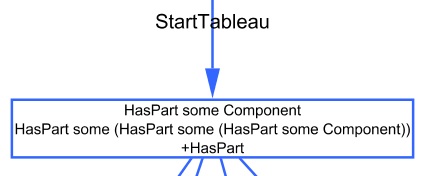
\includegraphics[scale=0.5]{premodelzondertransitivity}
\end{center}
\end{figure}

\end{frame}

\begin{frame}{Transitive roles example}

\begin{figure}[h]
\begin{center}
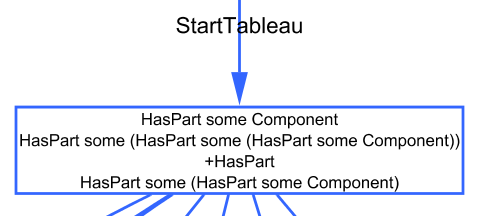
\includegraphics[scale=0.5]{premodelmettransitivity}
\end{center}
\end{figure}

\end{frame}

\begin{frame}{Role hierarchies}

\begin{table}[h]
\begin{center}
\begin{tabular}{l c}
LoTREC connective & \texttt{subrole} $C D$ \\
LoTREC display & $C subrole of D$ \\
\end{tabular}
\end{center}
\end{table}

\begin{table}[h]
\begin{center}
\begin{tabular}{l l}
TBox & $\exists{}Painted.Painting$ \\
ABox & $\forall{}Created.\neg{}Painting$ \& $Painted\sqsubseteq{}Created$ \\
\\
LoTREC input & \texttt{input tbox some Painted Painting} \\
 & \texttt{add only Created not Painting}\\
 & \texttt{subrole Painted Created} \\
\end{tabular}
\end{center}
\end{table}

\end{frame}

\begin{frame}{Role hierarchies example}

\begin{figure}
\begin{center}
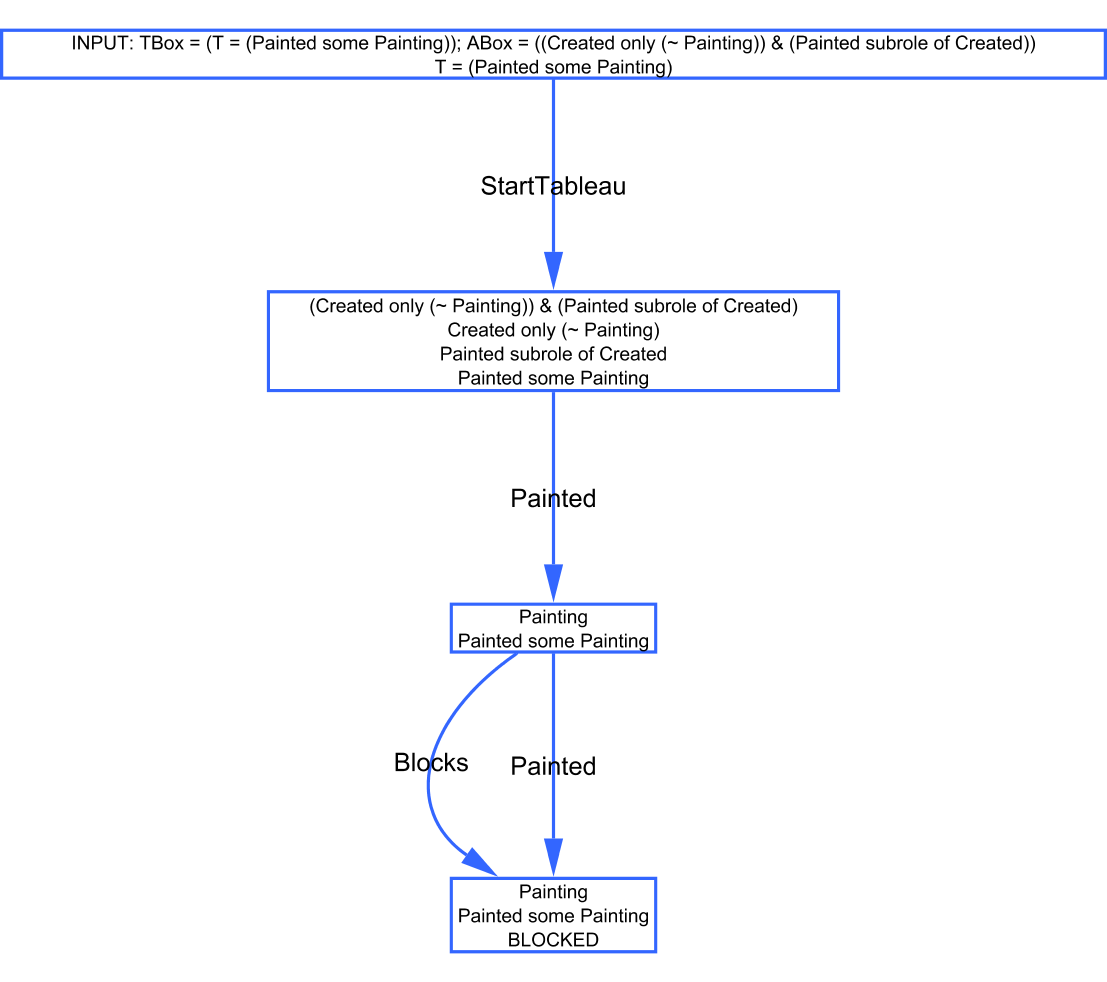
\includegraphics[scale=0.24]{premodelzondersubrole}
\end{center}
\end{figure}

\end{frame}

\begin{frame}{Role hierarchies example}

\begin{figure}
\begin{center}
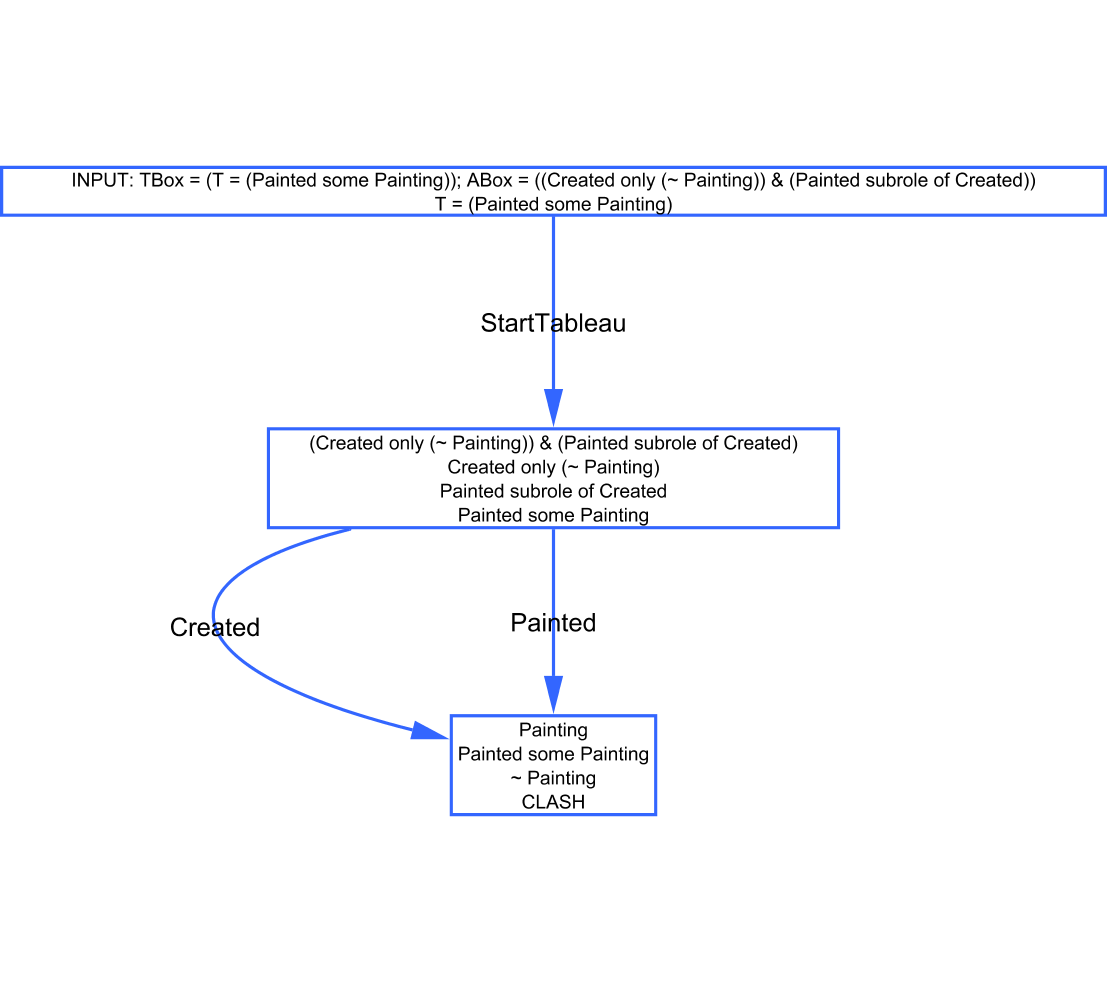
\includegraphics[scale=0.27]{premodelmetsubrole}
\end{center}
\end{figure}

\end{frame}


%\section{Conclusion}

\begin{frame}{Conclusions}
\begin{itemize}
\item LoTREC \frownie
\item Trial and Error Method \frownie
\item Finding a Wrong Blocking example \frownie
\item No Sudoku \frownie
\item No Sudoku competition results? \frownie
\end{itemize}
 
\end{frame}

\end{document}


